\chapter{Ergebnisse}
%
Die Klassifizierung des Zustandes der menschlichen Retina anhand von OCT
Aufnahmen in 4 Klassen (gesund + 3 Erkrankungen) lässt sich mit Hilfe des
maschinellen Lernens mit einer Genauigkeit von bis zu $\SI{90}{\percent}$
durchführen. Eine Lösung dieser Aufgabe, wie sie in dieser Arbeit beschrieben
ist, erfordert allerdings eine sehr hohe Rechenkapazität. Der verwendete
Datensatz liefert mit etwa $90\,000$ Bildern in sehr guter Auflösung eine
ausreichende Statistik, um gute Ergebnisse zu erzielen.
Die Hauptarchitektur eines CNN zeigt hierbei mit Abstand die beste
Genauigkeit. Nach etwa 40 Epochen lässt sich mit diesem Netz ein
Modell generieren, welches 4 Klassen mit einer Genauigkeit von
$\SI{90}{\percent}$ unterscheiden kann. Durch die Architektur können so Bilder
verschiedener Größen und Datensätze unterschiedlicher Verteilungen zur
Vorhersage verwendet werden. Durch ausreichende Regularisierung treten keine
Effekte von Übertraining auf, wie in Abbildung~\ref{fig:hist} zu sehen
ist.
%
\begin{figure}[h!]
  \subcaptionbox{Genauigkeit\label{fig:gen}}{\centering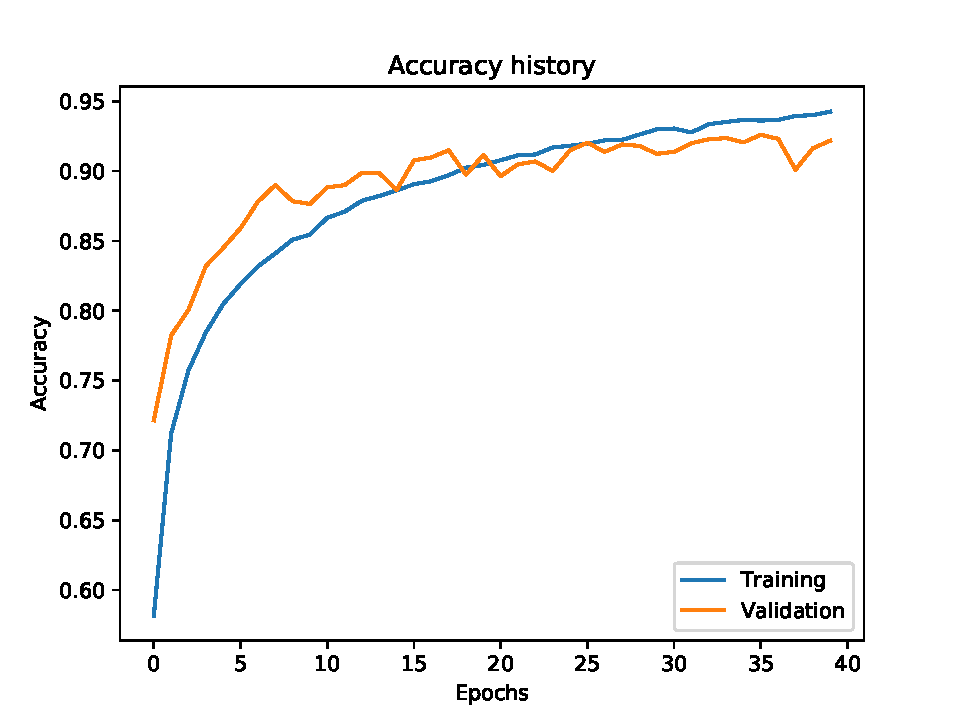
\includegraphics[width=0.5\linewidth]{Plots/accuracy_history_smaller.pdf}}
  \subcaptionbox{Verlustfunktion\label{fig:lo}}{\centering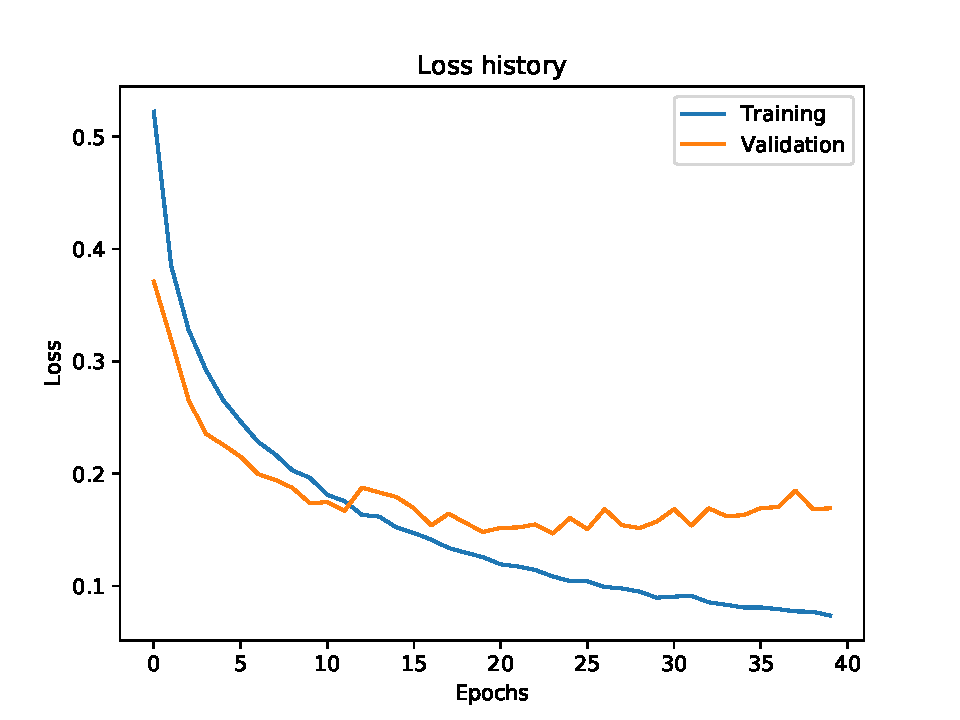
\includegraphics[width=0.5\linewidth]{Plots/loss_history_smaller.pdf}}
  \caption{Die Genauigkeit \protect\subref{fig:gen}, sowie die Verlustfunktion \protect\subref{fig:lo} der Hauptarchitektur des CNN. Es zeigen sich hier nach 40 Epochen keine Anzeichen für ein Übertraining.}
  \label{fig:hist}
\end{figure}
%
Betrachtet man Beispiele für die Klassen CNV, DRUSEN und NORMAL, deren
Trennung für das Netz am schwierigsten ist, so fällt auf, dass es sich hierbei
um Bilder handelt, die auch für Menschen schwierig zu trennen sind. Das Netz
erreicht allerdings mit der oben beschriebenen Genauigkeit eine Präzision, die
weit über der eines ungelernten Auges liegt. Ärzte hingegen erreichen
Genauigkeiten, die noch über dem hier erreichten Wert liegen.
\newpage
Eine Genauigkeit von $\SI{90}{\percent}$ durch Bilderkennung auf 4 Klassen zu
erreichen, stellt allerdings eine sehr optimistisch stimmende Leistung dar.
Diese liegt weit über dem Zufall von $\SI{25}{\percent}$.
Ein Vergleich mit der Genauigkeit der Diagnose der Erkrankung CNV durch
Mediziner zeigt, dass die hier für diese Klasse erreichten $\SI{93}{\percent}$
über der in einer Studie~\cite{CNV} erreichten Genauigkeit von
$\SI{86.5}{\percent}$ liegen.
%
\begin{figure}[h!]
  \subcaptionbox{Verwirrungsmatrix CNN\label{fig:conf}}{\centering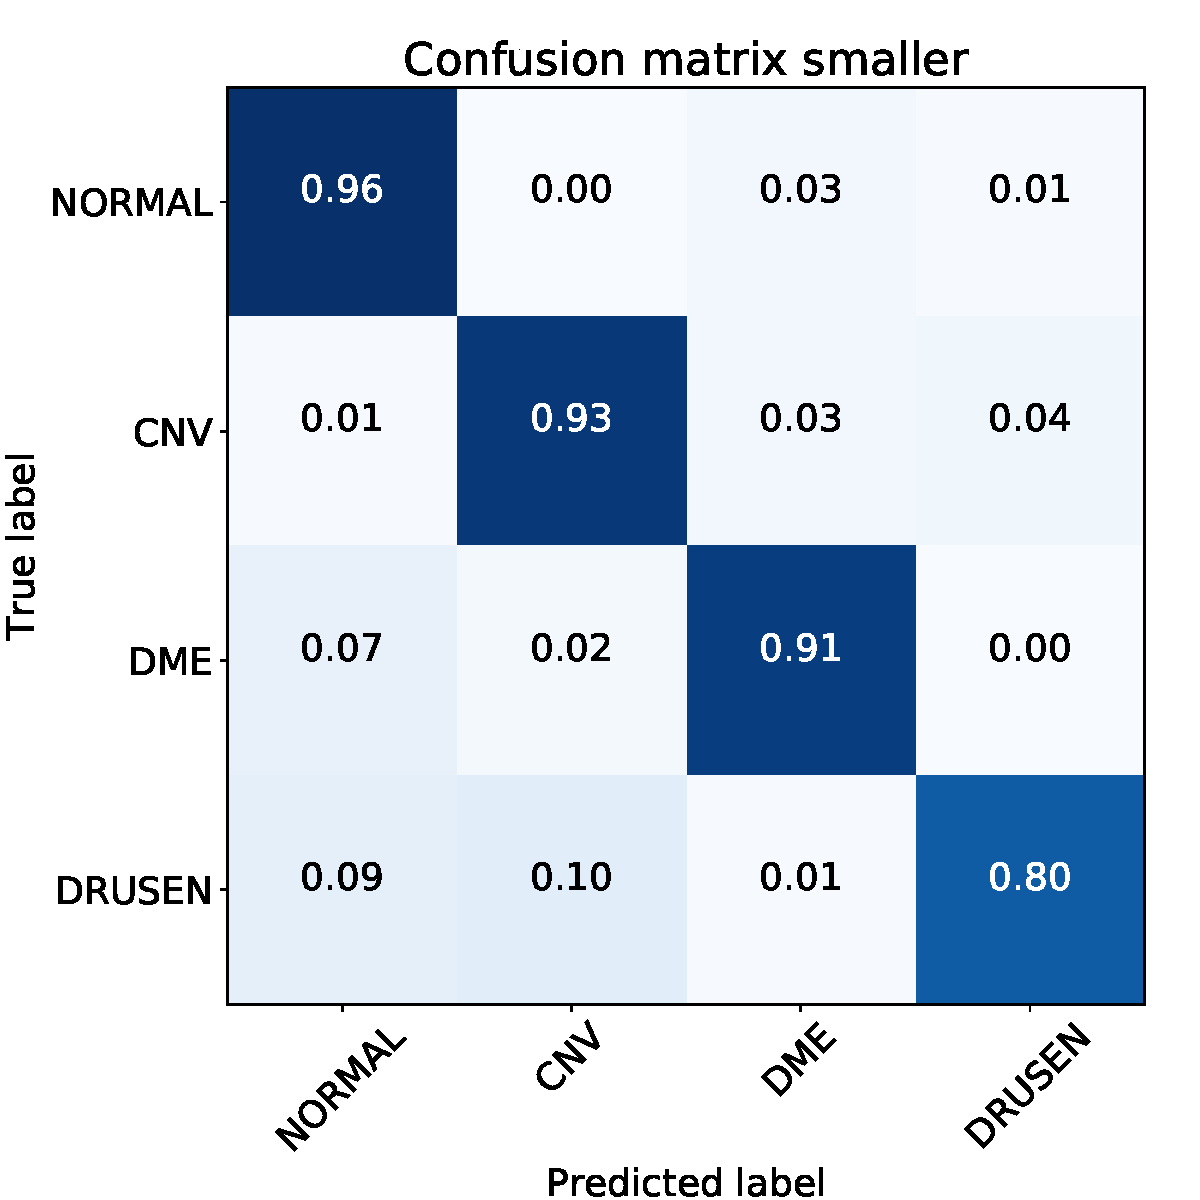
\includegraphics[width=0.4\linewidth]{Plots/confusion_matrix_smaller.pdf}}
  \subcaptionbox{Verteilung des Outputs des CNN für ein Validierungssample\label{fig:out}}{\centering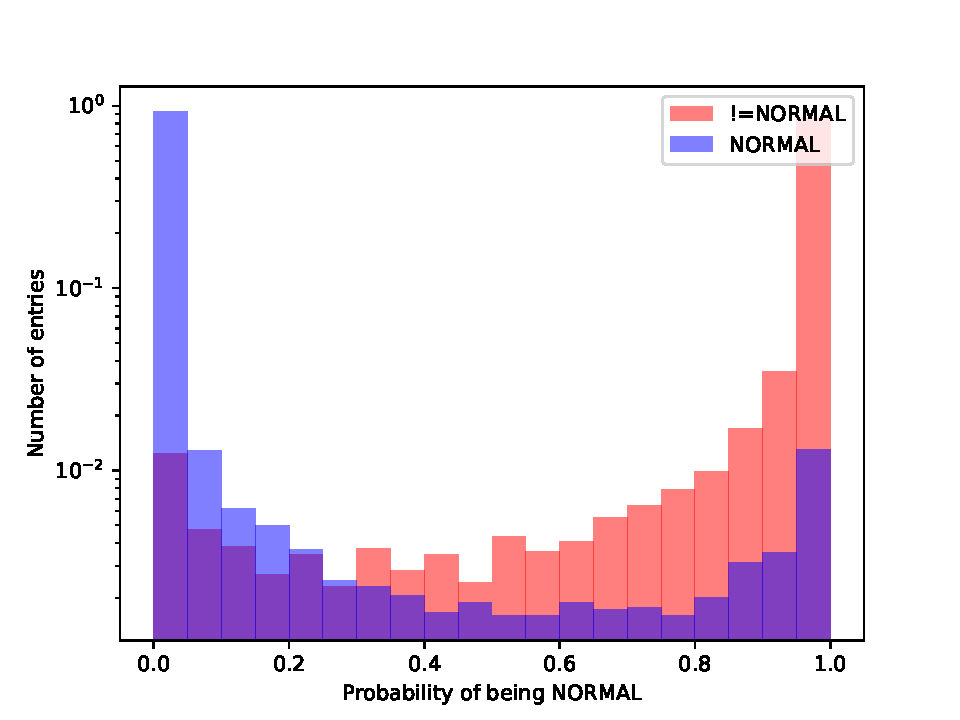
\includegraphics[width=0.55\linewidth]{Plots/NORMAL_or_not_log_smaller.pdf}}
  \subcaptionbox{Verwirrungsmatrix Alternativmethode\label{fig:conf_alt}}{\centering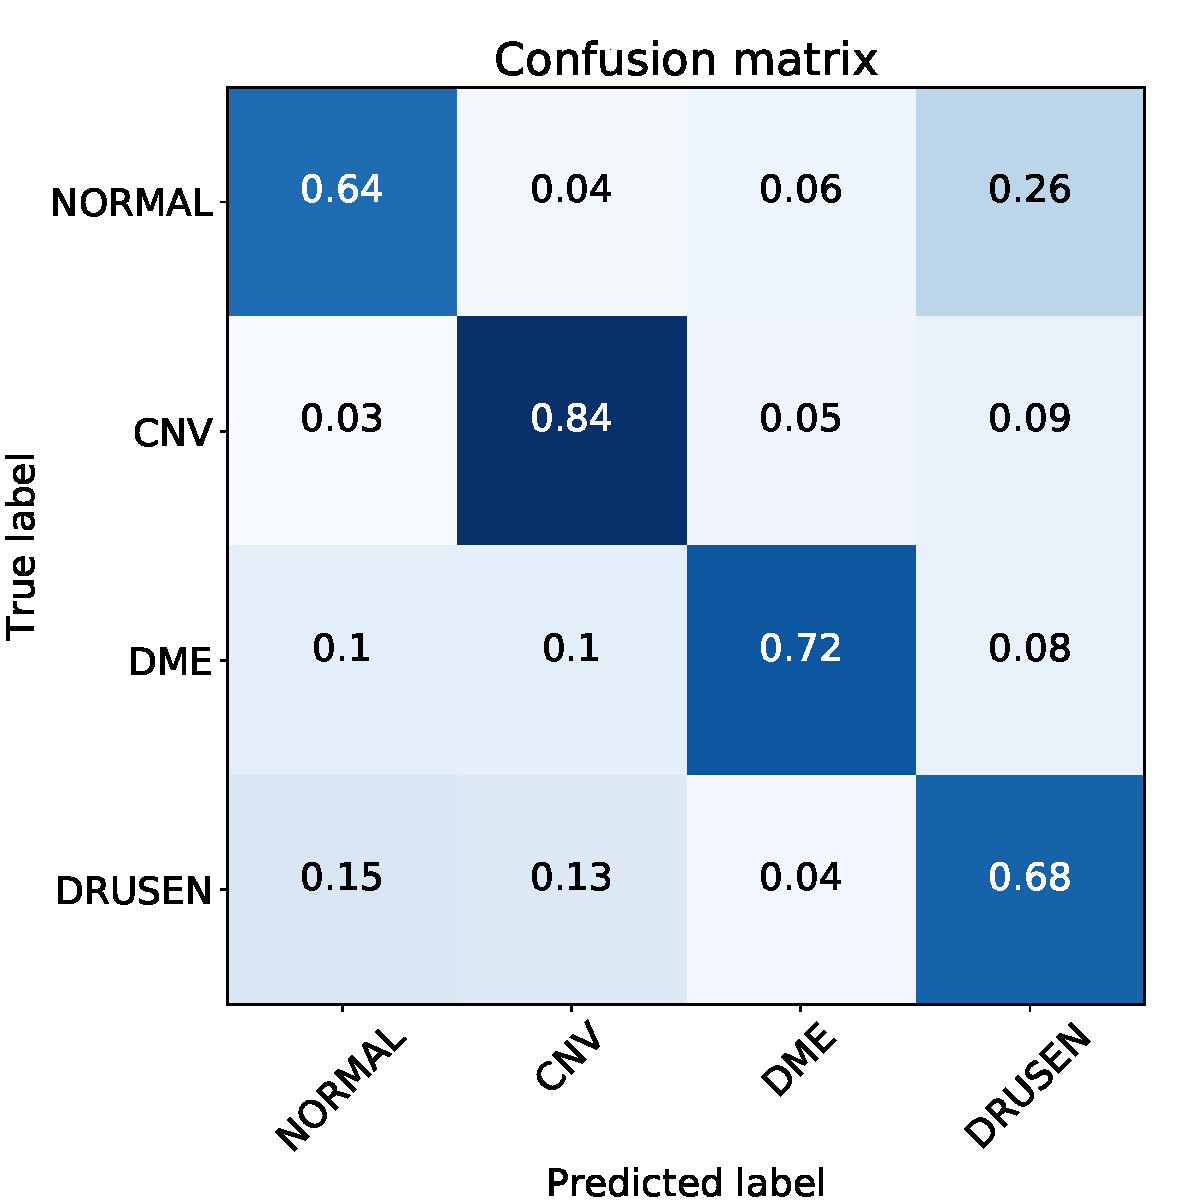
\includegraphics[width=0.4\linewidth]{Plots/confusionmatrix6test.pdf}}
  \subcaptionbox{Verlauf der Genauigkeit für die Alternativmethode\label{fig:acc_alt}}{\centering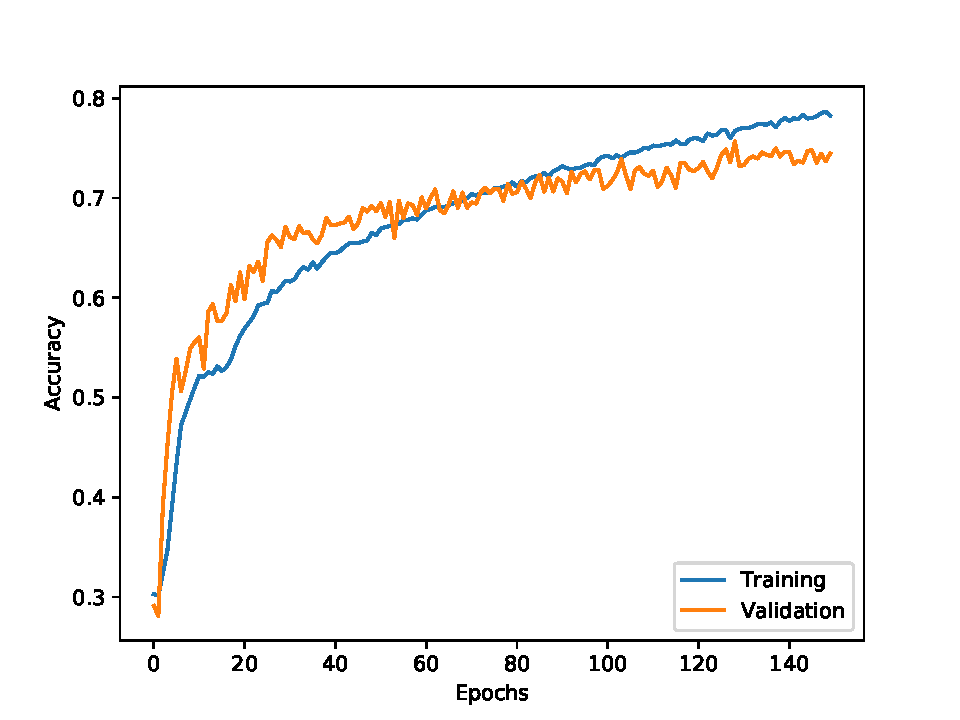
\includegraphics[width=0.55\linewidth]{Plots/accuracyhistory6.pdf}}
  \caption{Die Verwirrungsmatrix \protect\subref{fig:conf}
  \protect\subref{fig:conf_alt}, sowie der Output \protect\subref{fig:out} und
  der verlauf der Trainingsgenauigkeit \protect\subref{fig:acc_alt} der
  Hauptarchitektur des CNN, sowie der flachen alternativen Netzstruktur. Die
  Verwirrungsmatrix~\protect\subref{fig:conf} zeigt sehr hohe Genauigkeiten für
  die einzelnen Klassen, auch im Vergleich zur
  Alternativmethode~\protect\subref{fig:conf_alt}. Der Verlauf der Genauigkeit~\protect\subref{fig:acc_alt} zeigt allerdings, dass ein längeres Trainieren ins Übertraining führt. Der Output~\protect\subref{fig:out} des Netzes zeigt ebenfalls eine gute Trennung der Krankheiten vom gesunden Auge.}
  \label{fig:erg}
\end{figure}
%
\newpage
Allerdings zeigt diese Arbeit auch, dass sich mit deutlich einfacheren
Architekturen funktionierende Modelle entwickeln lassen, deren Genauigkeit weit
über dem Zufall liegen. Insbesondere zeigt sich trotz starker Skalierung des
Datensatzes, was eine deutliche Verringerung der Rechenzeit
zur Folge hat, eine Lösung mit einem einfachen vollständig vernetzten Netz.
Dabei ist eine Genauigkeit von etwa $\SI{72}{\percent}$ möglich. Dies liegt
deutlich unterhalb dessen, was das CNN leisten kann und zeigt damit auch, dass
CNN auf diesem Datensatz deutlich effektiver sind. Die erreichten
$\SI{90}{\percent}$ Genauigkeit stellen damit ein sehr gutes Ergebnis dar.
Auch für die Alternativmethode zeigt sich in Abbildung~\ref{fig:conf}, dass die
Unterscheidung der Klasse DRUSEN von den Klassen NORMAL und CNV besonders
schwierig erscheint. Allerdings scheint die Präparation der Daten wie in
Abschnitt~\ref{sec:alter} beschrieben, dafür zu sorgen, dass insbesondere auch
gesunde Retinas in etwa $\SI{25}{\percent}$ der Fälle für DRUSEN gehalten
werden. Allgemein muss hier deutlich länger trainiert werden, um zu hohen
Genauigkeiten zu gelangen.
Abschließend lässt sich festhalten, dass CNN in der Bilderkennung sehr gute
Leistungen zeigen. Auch in der Medizin lassen sie sich im Zusammenhang mit
bildgebenden Verfahren bei ausreichend großen Datenmengen einsetzen. Ein
überwachtes Lernen wie es hier vorgenommen wurde, schließt allerdings neue
Effekte, andere Erkrankungen oder das Erkennen anderer Defekte aus, sodass sie
sich in der Praxis nur eingeschränkt einsetzen lassen. Das Netz kann lediglich
in die Klassen einordnen, die im Datensatz vorhanden sind. Für die Aufgaben, die
sie dabei erfüllen können zeigen sie allerdings sehr hohe Genauigkeiten.
